% Pentest_report.tex
\documentclass[a4paper]{article}

\usepackage[utf8]{inputenc}
\usepackage[spanish]{babel}
\usepackage{graphicx}
\usepackage{lmodern}
\usepackage[dvipsnames,svgnames]{xcolor}
\usepackage[margin=2cm,top=2cm, includefoot]{geometry}
\usepackage[most]{tcolorbox}
\usepackage{fancyhdr}
\usepackage[hidelinks]{hyperref}
\usepackage{parskip}
\usepackage{listings}
\usepackage{smartdiagram}


% Declaración de colores
\definecolor{greenPortada}{RGB}{105,168,79}

% Declaración de variables
\newcommand{\logoPortada}{../images/logo.png} 
\newcommand{\logoMaquina}{../images/jerry.png}
\newcommand{\machineName}{Jerry}

% Adicionales
% Ajuste de headheight recomendado por fancyhdr (evita el error "headheight is too small")
\setlength{\headheight}{60pt}
\addtolength{\topmargin}{-14.47495pt}

\pagestyle{fancy}
\fancyhf{}
\lhead{\includegraphics[width=2cm]{\logoPortada}}\rhead{\includegraphics[width=1.2cm]{\logoMaquina}}
\renewcommand{\headrulewidth}{3pt}
\renewcommand{\headrule}{\hbox to\headwidth{
\color{greenPortada}\leaders\hrule height \headrulewidth\hfill}}


% Comienzo del documento --------------------------------------------------------------------------

\begin{document}
\cfoot{\thepage}

% Creación de la portada --------------------------------------------------------------------------

\begin{titlepage}
\centering
\includegraphics[width=0.6\textwidth]{\logoPortada}\par\vspace{1cm}
{\LARGE \textbf{WRITE-UP}} \par\vspace{0.25cm}
        {\Huge\bfseries\textcolor{greenPortada}{Maquina \machineName}\par\vspace{1cm}}
\vfill
\includegraphics[width=\textwidth,height=6cm, keepaspectratio]{\logoMaquina}\par\vspace{0.5cm}
\vfill
\begin{tcolorbox}[colback=green!5!white,colframe=green!75!black]
 \centering
   {\Large Autor: Aarón Ibarra}\par\vspace{0.4cm}
   {\large Fecha: 18 de Noviembre de 2025}\par
\end{tcolorbox}\par\vspace{0.1cm}
\vfill
{\large Todos los derechos reservados.}
\vfill
\end{titlepage}

% Índice --------------------------------------------------------------------------

\clearpage
\tableofcontents
\clearpage

% Contenido del informe --------------------------------------------------------------------------

% Introducción --------------------------------------------------------------------------
        
\section{Introducción}
\vspace{0.2cm}

\subsection{Antecedentes}
{\textbf{\machineName}} es una maquina clásica de \href{https://hackthebox.com}{\textbf{\textcolor{blue}{HackTheBox}}} diseñada para quienes están comenzando en el hacking ético. Clasificada como Fácil, esta máquina se centra en la explotación de un servidor Apache Tomcat mal configurado, lo que permite al atacante aprovechar credenciales por defecto y acceder al Manager App del servidor. A partir de este acceso, el usuario puede desplegar un archivo .war malicioso para lograr ejecución remota de código y finalmente obtener una shell en el sistema. 
\vfill
\begin{figure}[h]
\centering
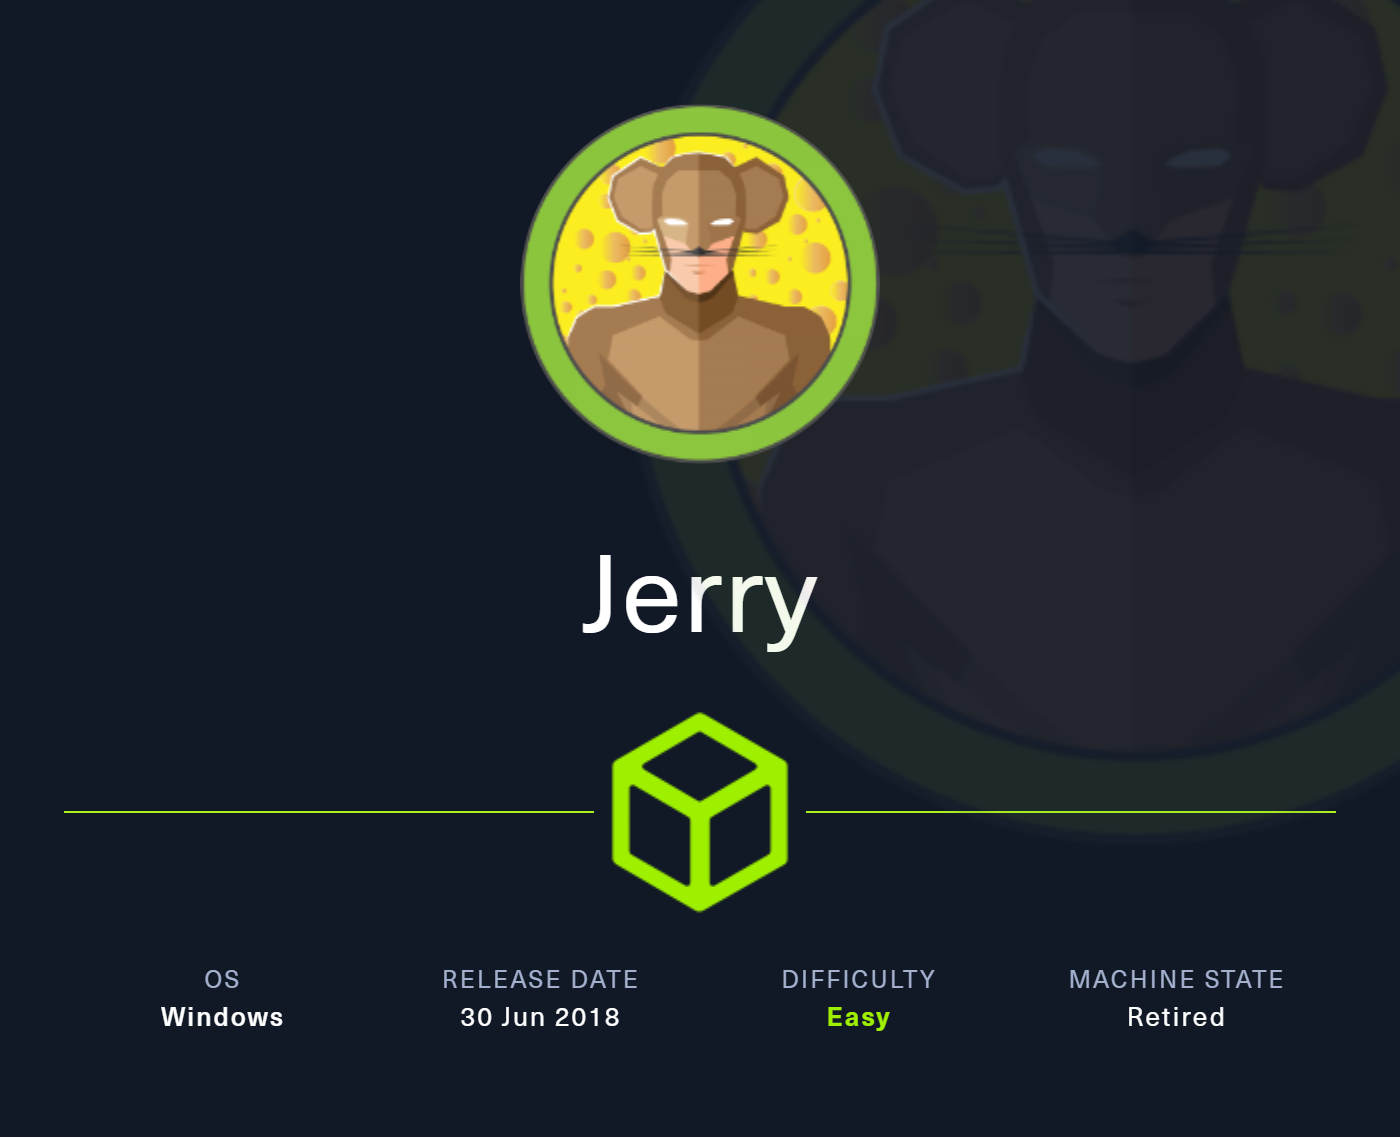
\includegraphics[width=0.55\textwidth]{../images/jerry-details.png}
\caption{Detalles de la máquina.}
\end{figure}
\vfill     
\begin{tcolorbox}[enhanced,attach boxed title to top center={yshift=-3mm,yshifttext=-1mm},
colback=blue!5!white,colframe=blue!75!black,colbacktitle=blue!80!black,
title=Dirección URL,fonttitle=\bfseries,
boxed title style={size=small,colframe=blue!50!black} ]
\centering
\href{https://app.hackthebox.com/machines/jerry}{\color{blue}{https://app.hackthebox.com/machines/jerry}}
\end{tcolorbox}
\vfill
        
\subsection{Objetivos}
En este ejercicio se pretende recorrer todo el ciclo de un ataque, desde la enumeración inicial hasta conseguir acceso con privilegios elevados.
\vfill
\begin{figure}[h]
\centering
\smartdiagramset{border color=none,
set color list={blue!50!cyan,green!60!lime,orange!50!red,red!80!black}, back arrow disabled=true}
\smartdiagram[flow diagram:horizontal] 
{Detectar un panel de administración expuesto, Identificar credenciale por defecto en Tomcat, Subir un archivo .war para obtener RCE, Crear una webshell desde el Manager App}
\caption{Fases del ataque realizadas en la máquina \machineName.}
\end{figure}
\vfill
%\begin{figure}[h]
%\centering
%\smartdiagram[flow diagram:horizontal]
%{Reconocimiento para delimitar el alcance y contexto operativo,
%Escaneo y enumeración de servicios y dependencias,
%Explotación controlada para verificar vulnerabilidades,
%Postexplotación segura y documentación de hallazgos}
%\end{figure}
\clearpage
        
% Enumeración --------------------------------------------------------------------------

\section{Enumeración}
\subsection{Reconocimiento inicial}
Se inició un análisis preliminar para comprobar la accesibilidad del sistema objetivo desde la máquina atacante, empleando la herramienta \texttt{ping} para enviar paquetes ICMP y confirmar la conexión del equipo en la red.
\vspace{0.2cm}
\begin{figure}[h]
\centering

\includegraphics[width=0.6\textwidth]{../enumeration/ping.png}
\caption{Reconocimiento inicial sobre el sistema objetivo.} 
\end{figure}
\vfill

Tras localizar el sistema se realizó un escaneo de puertos con la herramienta \texttt{nmap} con el fin de identificar los servicios en ejecución y las versiones asociadas, registrándose los siguientes hallazgos.\vspace{0.2cm}

\begin{figure}[h]  
\centering
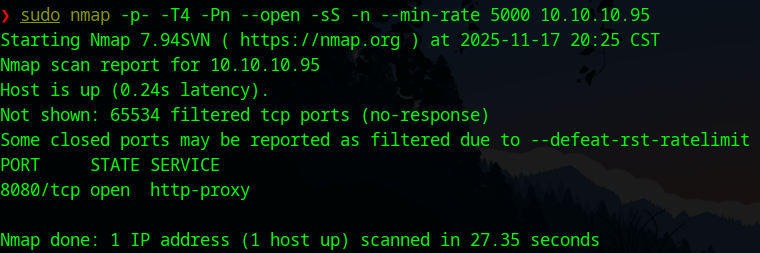
\includegraphics[width=.75\textwidth]{../enumeration/initial-nmap.png}
\caption{Escaneo inicial de puertos con nmap.}  
\end{figure}
\vfill

\subsection{Enumeración de servicios} A continuación, se procedió a una enumeración más detallada de los servicios identificados en el escaneo inicial, con el fin de obtener información adicional sobre sus configuraciones y posibles vulnerabilidades asociadas.
\vspace{0.2cm}

\begin{figure}[h]
\centering
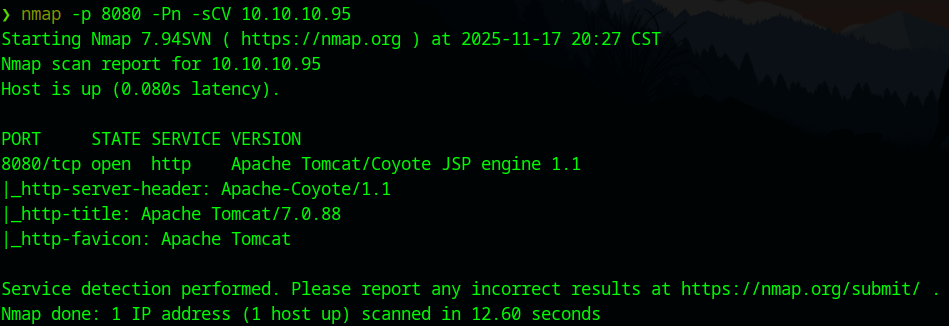
\includegraphics[width=.8\textwidth]{../enumeration/nmap-services.png}
\caption{Enumeración detallada de los servicios con nmap.}
\end{figure}
\vfill
\clearpage
        
% Explotación --------------------------------------------------------------------------
       
\section{Explotación}
Después de la enumeración inicial, se identificó que el servidor exponía un servicio web en el puerto 8080, correspondiente a Apache Tomcat.
Al acceder a dicho puerto, el servidor respondió con la siguiente página.\vspace{0.2cm}

\begin{figure}[h]
\centering              

\includegraphics[width=1\textwidth]{../enumeration/web.png}
\caption{Página de inicio del servidor Apache Tomcat.}
\end{figure}
\vfill

Posteriormente, se exploraron las distintas aplicaciones web desplegadas en el servidor, encontrándose la aplicación Manager App, que permite la gestión de aplicaciones web en Tomcat. Al intentar acceder a esta aplicación, se solicitó autenticación mediante un formulario de login.\vspace{0.2cm}

\begin{figure}[h]
\centering
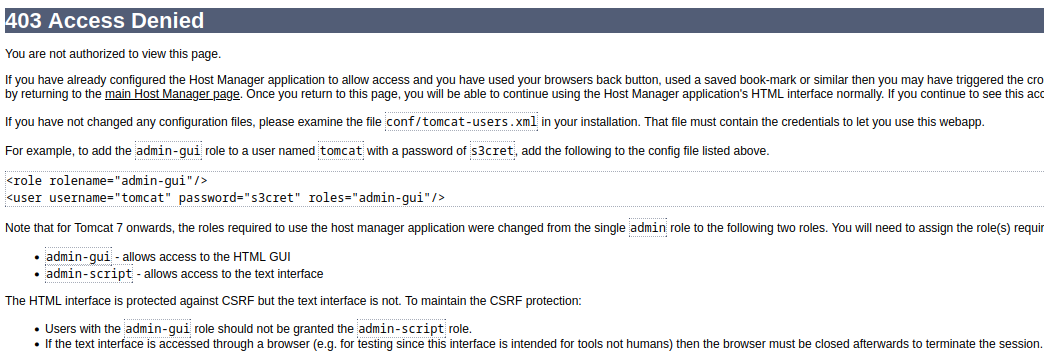
\includegraphics[width=1\textwidth]{../enumeration/403.png}
\caption{Intento de acceso al Manager App sin credenciales.}
\end{figure}
\vfill
\clearpage

Dado que Tomcat suele mantenerse con configuraciones inseguras, se probaron credenciales por defecto como admin:admin y tomcat:tomcat. Finalmente, el acceso al Manager App se consiguió con las credenciales tomcat:s3cret.\vspace{0.2cm}

\begin{figure}[h]
\centering
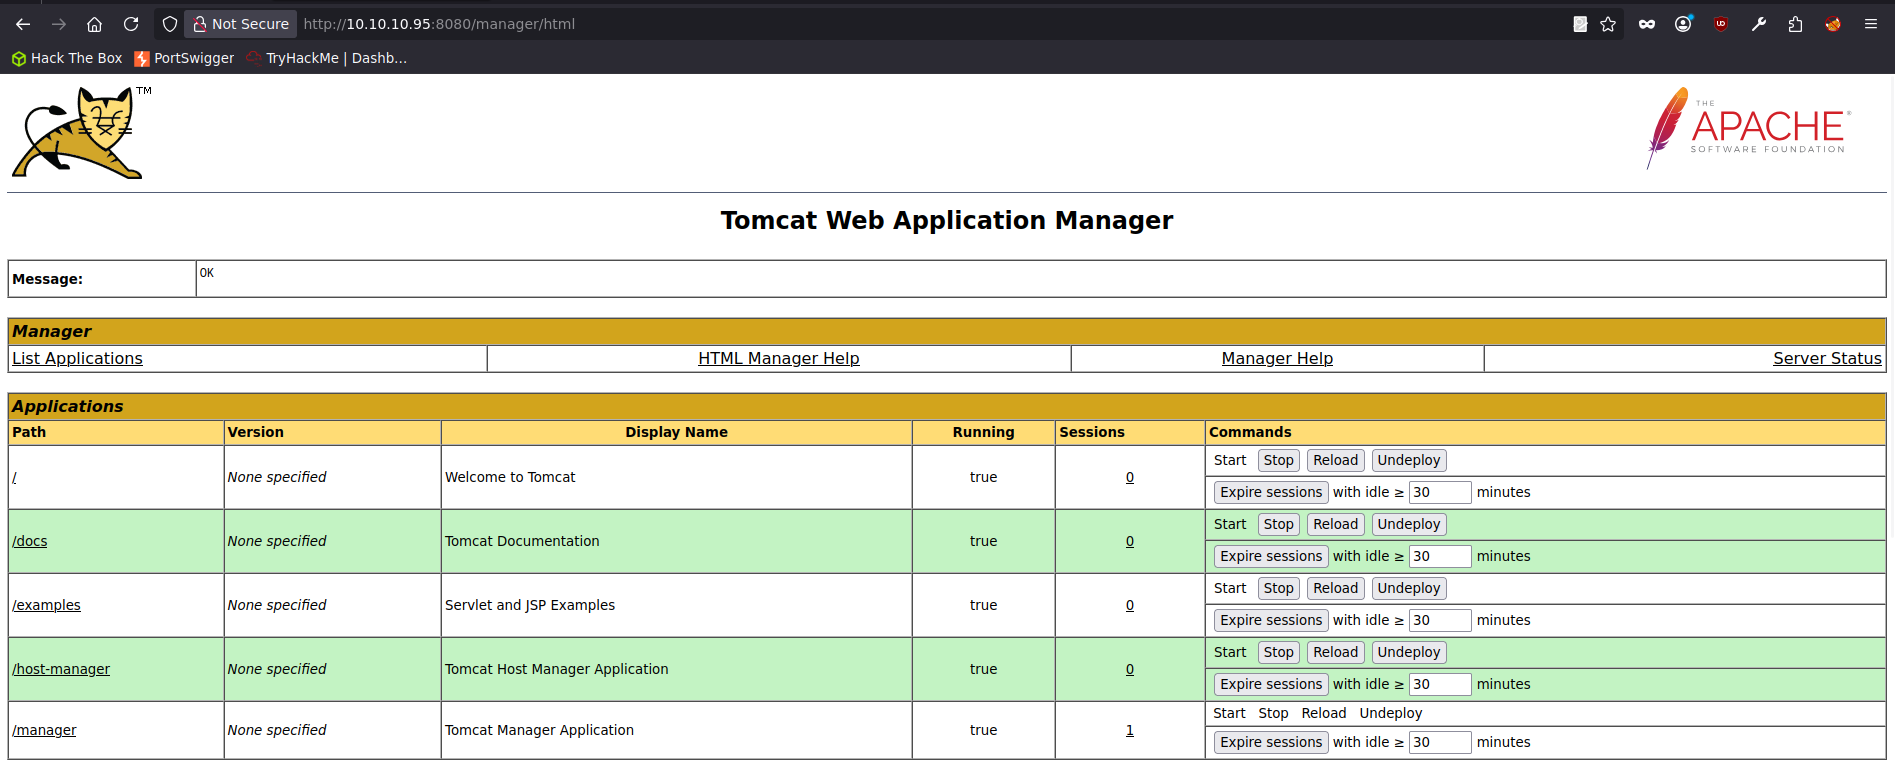
\includegraphics[width=1\textwidth]{../enumeration/manager.png}
\caption{Acceso exitoso al Manager App con credenciales por defecto.}
\end{figure}
\vspace{0.2cm}
Con acceso al Manager App, se procedió a desplegar un archivo .war malicioso para lograr ejecución remota de código (RCE) en el servidor. Se utilizó la herramienta \texttt{msfvenom} para generar un payload adecuado, que fue empaquetado en un archivo .war listo para ser subido al servidor.\vspace{0.2cm}

\begin{figure}[h]
\centering

\includegraphics[width=.9\textwidth]{../exploits/msfvenom.png}
\caption{Generación del archivo .war malicioso con msfvenom.}   
\end{figure}
|\vfill

\clearpage

Finalmente, se subió el archivo .war a través del Manager App y se inició un listener en la máquina atacante para capturar la conexión inversa. Al acceder a la URL correspondiente al payload desplegado, se logró obtener una shell remota en el sistema objetivo, confirmando así la explotación exitosa de la vulnerabilidad.\vspace{0.2cm}
\begin{figure}[h]
\centering 
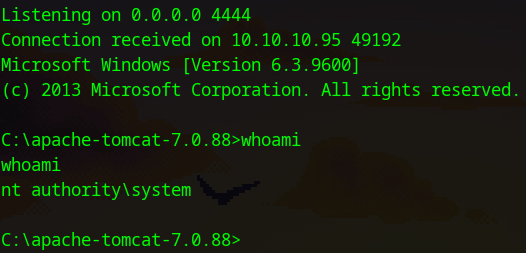
\includegraphics[width=.6\textwidth]{../exploits/jeje.png}
\caption{Obtención de shell remota en el sistema objetivo.}
\end{figure}

%\begin{figure}[h]
%\centering
%
\includegraphics[width=.9\textwidth]{images/exploitation.png}
%\caption{Obtención de shell remota en el sistema objetivo.}
%\end{figure}
%\vspace{0.2cm}  
\end{document}